\documentclass{a0poster}
\usepackage{fancytikzposter} 
 
\usepackage[T1]{fontenc} 
\usepackage[cp1251]{inputenc}
\usepackage[russian]{babel}
\usepackage{graphicx}
\usepackage{graphics}
\usepackage{amssymb}
\usepackage{mathtext}
\usepackage{caption}
\usepackage{subcaption}
\usepackage{setspace}
\usepackage{amsmath}
\usepackage{amsthm}
\usepackage{lscape}
\usepackage{makecell}
\usepackage{multirow}
\usepackage{ulem}
\usepackage{indentfirst}
\usepackage{enumerate}

\usepackage[margin=\margin cm, paperwidth=84.1cm, paperheight=118.9cm]{geometry}

%%%%% --------- Change here if you want ---------- %%%%%
%% margin for the geometry package, must be changed before using the geometry package
%% default value is 4cm
% \setmargin{4}

%% the space between the blocks
%% default value is 2cm
% \setblockspacing{2}

%% the height of the title stripe in block nodes, decrease it to save space
%% default value is 3cm
% \setblocktitleheight{3}

%% the number of columns in the poster, possible values 2,3
%% default value is 2
% \setcolumnnumber{3}

%% the space between two or more groups of authors from different institutions
%% used in \maketitle
% \setinstituteshift{10}

\usetemplate{3}

%% components of the templates
%% (the maximal possible numbers are mentioned as the parameters)
% \usecolortemplate{4}
% \usebackgroundtemplate{5}
% \usetitletemplate{2}
% \useblocknodetemplate{5}
% \useplainblocktemplate{4}
% \useinnerblocktemplate{2}


%% the height of the head drawing on top 
%% applicable to templates N3, 4 and 5
 \setheaddrawingheight{23}


%% change the basic colors
%\definecolor{myblue}{HTML}{008888} 
%\setfirstcolor{myblue}% default 116699
%\setsecondcolor{gray!80!}% default CCCCCC
%\setthirdcolor{red!80!black}% default 991111

%% change the more specific colors
\setbackgrounddarkcolor{colorone!70!black}
% \setbackgroundlightcolor{colorone!70!}
% \settitletextcolor{textcolor}
% \settitlefillcolor{white}
% \settitledrawcolor{colortwo}
% \setblocktextcolor{textcolor}
% \setblockfillcolor{white}
% \setblocktitletextcolor{colorone}
% \setblocktitlefillcolor{colortwo} %the color of the border
% \setplainblocktextcolor{textcolor}
\setplainblockfillcolor{colorone!10!}
% \setplainblocktitletextcolor{textcolor}
\setplainblocktitlefillcolor{colorone!60!}
% \setinnerblocktextcolor{textcolor}
% \setinnerblockfillcolor{white}
% \setinnerblocktitletextcolor{white}
% \setinnerblocktitlefillcolor{colorthree}

%% changing the fonts
%\usepackage{cmbright}

\renewcommand\normalsize{\fontsize{32}{39.8pt}\selectfont}

%% add your packages here
\usepackage{hyperref}

\title{ Stability loss of the trivial solution of boundary-value problem with \\ linear deviate 
in boundary condition }
\author{ \textit{ Leonid Ivanovsky$^{1,2}$, Sergey Kaschenko$^{1,3}$  } \\
\\
\textit{ $^{1}$P.G. Demidov Yaroslavl State University } \\
\textit{ $^{2}$Scientific Center in Chernogolovka of Russian Academy of Sciences } \\
\textit{ $^{3}$National Research Nuclear University MEPhI }
}

\begin{document}

%%%%% ---------- the background picture ---------- %%%%%
%% to change it modify the macro \BackgroundPicture
\ClearShipoutPicture
\AddToShipoutPicture{\BackgroundPicture}

\noindent % to have the picture right in the center
\begin{tikzpicture}
  \initializesizeandshifts
  % \setxshift{15}
  % \setyshift{2}

  %% the title block, #1 - shift, the default value is (0,0), #2 - width, #3 - scale
  %% the alias of the title block is `title', so we can refer to its boundaries later
  \ifthenelse{\equal{\template}{1}}{ 
    \titleblock{47}{1}
  }{
    \titleblock{47}{1.5}
  }

  %% a logo can be added to the title block
  %% #1 - anchor relative to the title block, #2 - shift, #3 - width, #3 - file name
  % \ifthenelse{\equal{\template}{2}}{ 
  %   \addlogo[south west]{(2,0)}{6cm}{unibz_b.png}
  % }{
  %   \addlogo[south west]{(2,0)}{6cm}{unibz_w.png}
  % }

  %%%%%%%%%% ------------------------------------------ %%%%%%%%%%
  \blocknodew{37}{ Boundary-value problem } %
  {
	\begin{equation}\label{ivanovsky-eq1}
		\dot{u} = \beta u'' - \gamma u,	
	\end{equation}
	\begin{equation}\label{ivanovsky-eq2}
		u'\mid_{x=0} \, = 0, \quad u'\mid_{x=1} \, = \alpha\,u\mid_{x=x_0},
	\end{equation}	
	
	$$ \alpha, \gamma \in \mathbb{R}, \quad \beta > 0, \quad x_0 \in [0, 1]. $$
  } 

  \blocknodew{37}{  } %
  {
	$$ w(x) = c\,\mbox{ch}(\mu\, x), $$
	$$ x = 1: \quad \mu \, \mbox{sh} \mu = \alpha \, \mbox{ch} (\mu\, x_0), $$
	
	$$ \mu = \sqrt{\lambda}, \quad \lambda \in \mathbb{C}. $$
  } 

	\blocknodew[($(currenty)+(19.5,0)$)]{76}{ Numerical result: potential $\alpha_{cr}$ } %
  { 
  
  	\bigskip
	
	\hspace{-7.5cm}
	\begin{minipage}[h]{0.68\linewidth}
	\center{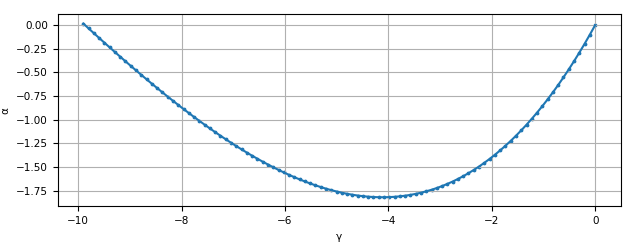
\includegraphics[width=0.68\linewidth]{0,0.png} \\ a) $ x_0 = 0 $ }
	\end{minipage}	
	\hspace{-14cm}
	\begin{minipage}[h]{0.68\linewidth}
	\center{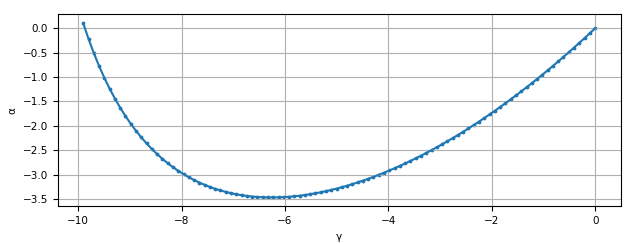
\includegraphics[width=0.68\linewidth]{0,45.png} \\ b) $ x_0 = 0{,}45 $ }
	\end{minipage}
	
	~\\
	
	\hspace{-7.5cm}
	\begin{minipage}[h]{0.68\linewidth}
	\center{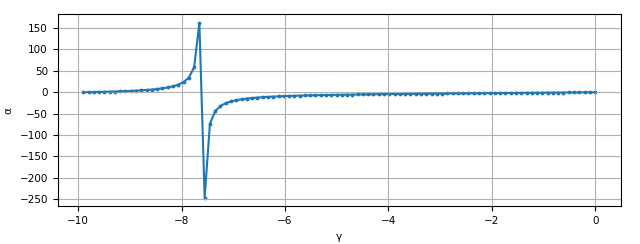
\includegraphics[width=0.68\linewidth]{0,57.png} \\ c) $ x_0 = 0{,}57 $ }
	\end{minipage}	
	\hspace{-14cm}
	\begin{minipage}[h]{0.68\linewidth}
	\center{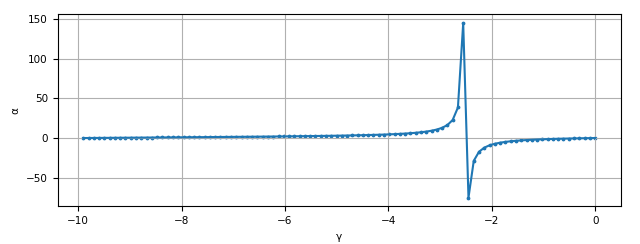
\includegraphics[width=0.68\linewidth]{0,99.png} \\ d) $ x_0 = 0{,}99 $ }
	\end{minipage}
  
  }
  
  \blocknodew[($(currenty)$)]{76}{ Numerical result: eigenfunctions } %
  { 
	
	\hspace{-7.5cm}
	\begin{minipage}[h]{0.5\linewidth}
	\center{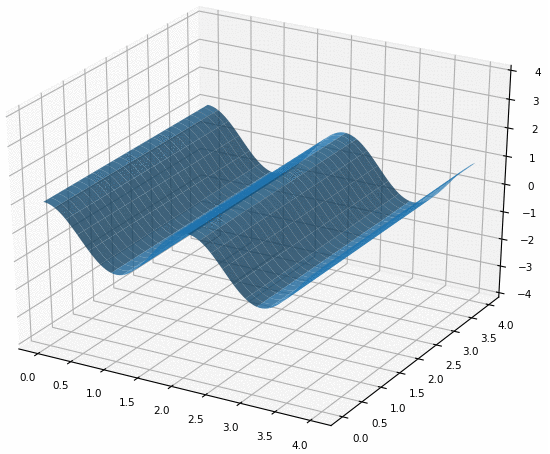
\includegraphics[width=0.5\linewidth]{1.png} }
	\end{minipage}	
	\hspace{-11.5cm}
	\begin{minipage}[h]{0.5\linewidth}
	\center{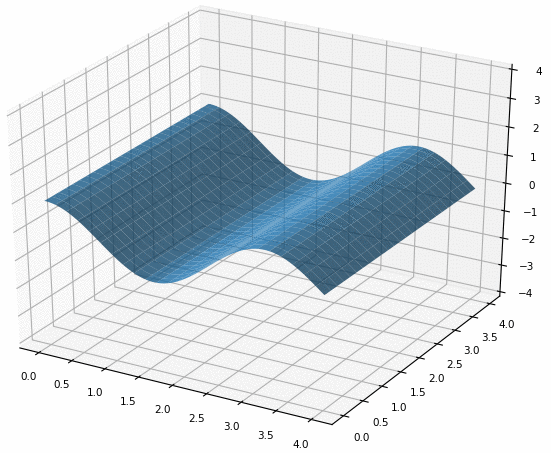
\includegraphics[width=0.5\linewidth]{2.png} }
	\end{minipage}
	\hspace{-11.5cm}
	\begin{minipage}[h]{0.5\linewidth}
	\center{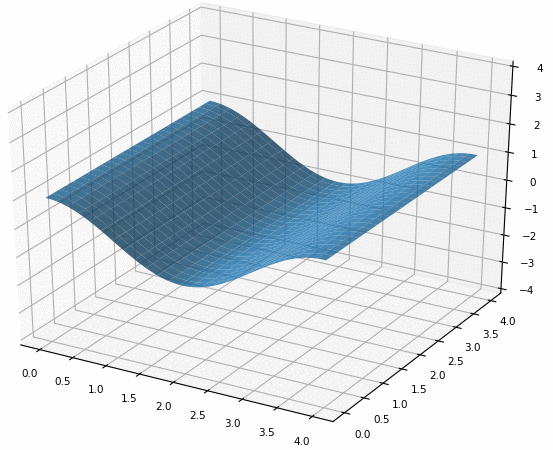
\includegraphics[width=0.5\linewidth]{3.png} }
	\end{minipage}
  
  }

  %%%%%%%%%%%%% NEW COLUMN %%%%%%%%%%%%%%% 
  \startsecondcolumn 

%%%%%%%%%% ------------------------------------------ %%%%%%%%%%
  \blocknodew{37}{ Eigenvalue problem } %
  {
	
	$$ u(x, t) = w(x)\,\mbox{exp}\left( \lambda - \frac{\gamma}{\beta} \right)t $$
	
    \vspace{1.5cm}	
	
	\begin{equation}\label{ivanovsky-eq3}
		w'' - \lambda w = 0,
	\end{equation}
	\begin{equation}\label{ivanovsky-eq4}
		w'(0) = 0, \quad w'(1) = \alpha\,w(x_0).
	\end{equation}
	
  }

  \blocknodew{37}{ Main result } %
  {	
    
    \vspace{1.5cm}  
    
	\begin{minipage}{\linewidth}
        \coloredbox{colorthree!150!}{\textbf{Theorem:} Suppose $ x_0 \in [0, 1], \; \beta > 0, \; \gamma > 0 $. Then there exists $ \alpha=\alpha_{cr} $, for that $ \mbox{Re}(\lambda_{*}) = \dfrac{\gamma}{\beta} $ and for the rest eigenvalues of problem (3), (4) $ \mbox{Re}(\lambda) < \dfrac{\gamma}{\beta} $.}
     \end{minipage} 
     
     \vspace{1.5cm} 
     
  }
      
\vspace{0.35cm}

\end{tikzpicture}

\end{document}